\documentclass[11pt,letterpaper]{article}
\usepackage{amsmath}
\usepackage{amsfonts}
\usepackage{amssymb}
\usepackage{fullpage}
\usepackage{graphicx}
\usepackage[normalem]{ulem}
\usepackage{url}

\begin{document}

\begin{center}
\huge
\textsc{Smart Refrigerator Design Project}\\
\Large
\textsc{Progress Report I} \\
\vspace{.20cm}
\hrule
\vspace{.40cm}
\normalsize
Steven Strapp, Ben Reeves, Dustin Stroup \\
\today \\
\vspace{1cm}
\end{center}

\section{Updated Milestone Chart}
\begin{table}[h!]
\begin{center}
\begin{tabular}{| p{3.5 cm} | p{2 cm} | p{2 cm}| p{2 cm} | p{6 cm} | }
\hline
\textbf{Milestone} & \textbf{Scheduled Date} & \textbf{Assigned} & \textbf{Modified Date} & \textbf{Comments} \\
\hline
BeagleBoard \newline procured & February 10, 2012 & SS & NA & Complete \\
\hline
Angstrom operating system running on board & February 24, 2012 & DS & NA & Complete \\
\hline
Peripherals properly interfacing with \newline board & March \newline 02, 2012 & DS & March \newline 30, 2012 & Complete aside from temperature sensor. Was not considered in \newline original timeline. \\
\hline
Basic mobile UI, \newline suitable for \newline debugging & March \newline 09, 2012 & BR & NA & Complete \\
\hline
Basic base station UI, suitable for \newline debugging & March \newline 09, 2012 &SS & Complete & Completed basic GUI functionality. Backend storage / algorithms not implemented. \\
\hline
Database I/O \newline configured & March \newline 16, 2012 & DS &  March \newline 23, 2012 & \\
\hline
Testing and \newline integration of \newline temperature and \newline humidity sensor & March \newline 16,  2012 &SS & March 30, \newline 2012 & Partially complete. Tested using Arduino. Not integrated with \newline Beagleboard. \\
\hline
Database and web server hosted by\newline Beagleboard & March \newline 16, 2012 & DS & Complete & Running, access to SQL server needs to be configured.\\
\hline
\vdots & \vdots & \vdots & \vdots & \vdots \\
\hline
\end{tabular}
\end{center}
\end{table}

\begin{table}[h!]
\begin{center}
\begin{tabular}{| p{3.5 cm} | p{2 cm} | p{2 cm}| p{2 cm} | p{6 cm} | }
\hline
\textbf{Milestone} & \textbf{Scheduled Date} & \textbf{Assigned} & \textbf{Modified Date} & \textbf{Comments} \\
\hline

Beagleboard \newline touchscreen display procured & March \newline 16, 2012 & DS & NA & Supplier found via Dr. Mondragon, submitting purchase order. \\
\hline
Mobile application integrated with web server & March 30, 2012 &BR & & \\
\hline
User profiling and statistical analysis & March 30, 2012 & SS & & \\
\hline 
Shopping lists, item modification, basic settings & March 30, 2012 & DS & &\\
\hline
Updated base station UI & April 6, 2012 & SS & & \\
\hline
Updated mobile application & April 6, 2012 & BR & & \\
\hline
Improved robustness of mobile interface& April 13, 2012 & DS & & \\
\hline
Integration testing and system verification & April 13, 2012 & BR & & \\
\hline
System testing and demo preparation & April 20, 2012 & SS & & \\
\hline
\end{tabular}
\label {MilestoneTable}
\end{center}
\end{table}

\quad \newline \quad
\quad \newline \quad
\quad \newline \quad
\quad \newline \quad

\pagebreak[4]

\section{Current Milestones}
\begin{table}[h!]
\begin{center}
\begin{tabular}{| p{3.5 cm} | p{2 cm} | p{2 cm}| p{2 cm} | p{6 cm} | }
\hline
\textbf{Milestone} & \textbf{Scheduled Date} & \textbf{Assigned} & \textbf{Modified Date} & \textbf{Comments} \\
\hline
BeagleBoard \newline procured & February 10, 2012 & SS & NA & Complete \\
\hline
Angstrom operating system running on board & February 24, 2012 & DS & NA & Complete \\
\hline
Peripherals properly interfacing with \newline board & March \newline 02, 2012 & DS & March \newline 30, 2012 & Complete aside from temperature sensor. Was not considered in \newline original timeline. \\
\hline
Basic mobile UI, \newline suitable for \newline debugging & March \newline 09, 2012 & BR & NA & Complete \\
\hline
Basic base station UI, suitable for \newline debugging & March \newline 09, 2012 &SS & Complete & Completed basic GUI functionality. Backend storage / algorithms not implemented. \\
\hline
Database I/O \newline configured & March \newline 16, 2012 & DS &  March \newline 23, 2012 & \\
\hline
Testing and \newline integration of \newline temperature and \newline humidity sensor & March \newline 16,  2012 &SS & March 30, \newline 2012 & Partially complete. Tested using Arduino. Not integrated with \newline Beagleboard. \\
\hline
Database and web server hosted by\newline Beagleboard & March \newline 16, 2012 & DS & Complete & Running, access to SQL server needs to be configured.\\
\hline
Beagleboard \newline touchscreen display procured & March \newline 16, 2012 & DS & NA & Supplier found via Dr. Mondragon, submitting purchase order. \\
\hline
\end{tabular}
\end{center}
\end{table}

\quad \newline \quad
\pagebreak

\section{Next Milestones}
\begin{table}[h!]
\begin{center}
\begin{tabular}{| p{3.5 cm} | p{2 cm} | p{2 cm}| p{2 cm} | p{6 cm} | }
\hline
\textbf{Milestone} & \textbf{Scheduled Date} & \textbf{Assigned} & \textbf{Modified Date} & \textbf{Comments} \\
\hline
Mobile application integrated with web server & March 30, 2012 &BR & & \\
\hline
User profiling and statistical analysis & March 30, 2012 & SS & & \\
\hline
Database I/O \newline configured & March \newline 16, 2012 & DS &  March \newline 23, 2012 & \\
\hline
Peripherals properly interfacing with \newline board & March \newline 02, 2012 & DS & March \newline 30, 2012 & Complete aside from temperature sensor. Was not considered in \newline original timeline. \\
\hline
\end{tabular}
\end{center}
\end{table}

\section{Status}
\begin{itemize}
\item Preliminary version of mobile application and base station interface were developed. 
\item Next steps are to incorporate network interface into mobile application, and to add back-end processing and database interaction to base station application.
\item  Dr.\ Mondragon has located a supplier for the desired LCD display, a purchase order will be submitted shortly. 
\item The Beagleboard is running the webserver and python.
\end{itemize}

\section{Gantt Chart}
\begin{figure}[h!]
\begin{center}
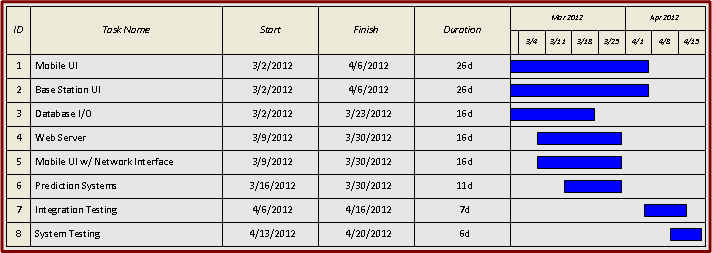
\includegraphics[scale=.6]{GanttChartI}
\end{center}
\end{figure}

\end{document}
